\documentclass[../main.tex]{subfiles}

\begin{document}

Due to the propagation delay of transactions in the network, not all nodes share the same vision of the Tangle at the same time.
This might lead to situations where the validation process lets multiple transactions in conflict with each other join the Tangle.
It is a fundamental assumption of the IOTA white paper that the Tangle itself can indeed contain conflicting transactions.
In case of a conflict, however, the nodes need to decide which transaction(s) should be considered valid, i.e., they need to come to a \emph{consensus} on those conflicting transactions.

In the original IOTA white paper this is solely achieved by consistently applying the tip selection algorithm (TSA), i.e., the mechanism used by (honest) nodes to select the transactions to approve, which currently uses a biased random walk. In case of a conflict, this bias will eventually leave all but one of the conflicting branches behind. However, this approach is not suited for our current vision of the Tangle, as conflict resolution is slow and it leads transactions that chose the ``wrong'' branch to be orphaned, creating the need for a large number of reattachments.


In this section we discuss a consensus mechanism  which we call Shimmer and that is a mechanism to achieve consensus that is robust against potential attacks. The Shimmer voting scheme is named after an extraordinary behavior seen in nature. Bees “synchronize” their movement to defend themselves against predators. They do this without any centralized entity, and only know when to “change their state” by observing the behavior of their peers. Individual autonomous agents that act according to some predefined rules can be found in many systems in nature, such as bees, ants, schools of fish and even in some areas of physics. Very simple rules can create incredibly complex features that, over time, manifest as emergent properties of a system. The Shimmer consensus mechanism works in the same way. Instead of trying to reconstruct the opinion of every other node, we care only about the opinions of a very small subset of nodes and let consensus be formed organically as an emergent property of the network.


More specifically the idea is that nodes query other nodes about their current opinion of the ledger, and adjust their own opinion over the course of several rounds based on the proportion of other opinions they have observed. Whilst the voting models have their limitations, they have been successfully applied in a wide range of engineering and economical applications~\cite{banisch2010, niu2015, przyby2011}, leading to the emerging science of sociophysics~\cite{castellano2009}. We describe two voting mechanisms where nodes communicate to each other to decide, in case of a conflict, which transaction(s) should be accepted in the Tangle.

For this section, we only consider algorithms that find consensus on the value of a single bit, i.e., of a single conflict. The result of this consensus process can then be used to mark a transaction as either \enquote{liked} or \enquote{disliked}.

So, the general idea is to let the nodes talk to each other in order to resolve the conflicts \textit{pro-actively}. The conflict resolution is performed starting from an initial opinion on the ledger status described as follows:
Consider a transaction $v$. If in a given interval a node does not see any other transaction spent from the same address, we say that the node \textit{likes} transaction $v$; otherwise, the node \textit{dislikes} $v$\footnote{It is important to note, that this rule does not include reattachments: If $v_1,\ldots ,v_k$ are all reattachments of the same transaction, we either like all or none of them.}.
The decision whether a transaction is liked or disliked must then be taken into account for the tip selection.
The most straightforward way of integrating this is to simply remove 
all the tips in the future cones of disliked transactions 
 from the tip selection.

After that, we periodically apply a voting scheme to every transaction in the Tangle where each node asks for the opinion of some of its neighbors. After the vote, a transaction is either definitely liked or definitely disliked by a node.
We would like to keep monotonicity in the sense that if a node likes $u$ then it likes any transaction $u$ approves, and if the node dislikes $v$ then it dislikes any transaction that approves $v$, see Fig.~\ref{f_voting_consist}.
To achieve this, we can safely assume that we can only like transaction~$v$ when we like all of its past cone, and if we dislike~$v$ then we dislike all of its future cone.

\begin{figure}
\begin{center}
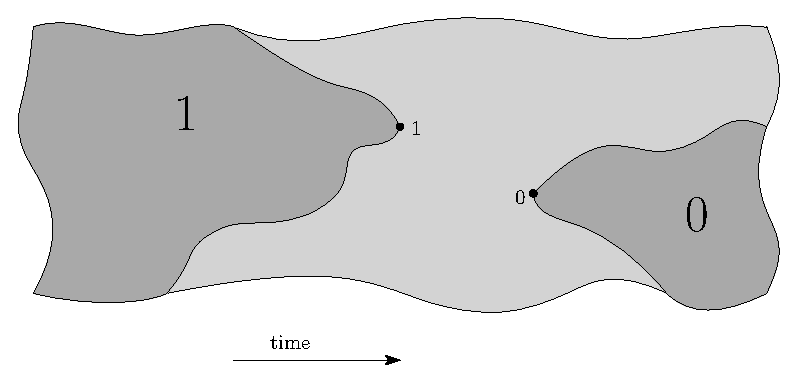
\includegraphics[width=0.75\textwidth]{voting_consist}
\caption{Votes must be monotonous}
\label{f_voting_consist}
\end{center}
\end{figure}

In the following two subsections, we will describe two voting mechanisms we are considering.
The first one, called \emph{Fast Probabilistic Consensus}~\cite{popov2019}, is certified by rigorous mathematical proofs; however, this solution requires nodes to accept connections from nodes which are not neighbors, and uses decentralized randomness, that needs to be acquired as part of an additional layer.
On the other hand, the cellular automaton approach of Section~\ref{s_cellular} does not have those requirements and seems to be faster from simulation results; however, this scheme lacks rigorous proofs and requires a stricter autopeering solution to avoid Eclipse attacks, and formation of \enquote{islands} of adversarial nodes.
The two solutions can be considered as different non-mutually exclusive implementations of the voting mechanism, and they can be used in combination to build a robust framework.

For more technical details, we refer the interested reader to the source code of our FPC simulator\footnote{\url{https://github.com/iotaledger/fpc-sim}}, as well the integration as a prototype version of FPC and the cellular automaton approach in \emph{GoShimmer}\footnote{\url{https://github.com/iotaledger/goshimmer}}. 

\end{document}
